\documentclass{article}

\usepackage{amsfonts}
\usepackage[colorlinks=true,citecolor=blue,urlcolor=cyan,linkcolor=red]{hyperref}
\usepackage{amssymb}
\usepackage{amsmath,amssymb,amscd,epsfig,amsfonts,rotating}
\usepackage{graphicx}
\usepackage{epsfig}
\usepackage{multirow}
\usepackage{booktabs}
\usepackage{bm}
\usepackage{url}
\usepackage[margin=1.5in]{geometry}

\newtheorem{def:def}{Definition}
\newtheorem{thm:thm}{Theorem}
\newtheorem{thm:lm}{Lemma}

\DeclareMathOperator*{\argmax}{arg \, max}
\DeclareMathOperator*{\var}{var}
\DeclareMathOperator*{\cov}{cov}
\newcommand{\bs}{\boldsymbol}

\title{Hierarchical Neural Model for Recommending Articles\\
		\Large{CS420 Coursework: Text Classification}}
\author{Runzhe Yang\\
{\small RzAlpaca, 5140309562} \\
{\small Shanghai Jiao Tong University}\\
{\small \textsf{yang\_runzhe@sjtu.edu.cn}}}
\begin{document}
\maketitle

\begin{abstract}
In this coursework, the author implemented various advanced neural network architectures for the text classification task. Based on several successful convolutional neural networks (CNN), the author proposed a novel hierarchical neural model, which is compatible with inherent hierarchical properties of documents. The experiment shows that the proposed model outperforms conventional character-level CNNs on AUC criterion. Even without sufficient training, the stacking tricks integrating existing models help further improve the final performance in kaggle competition.
\end{abstract}

\section{Introduction}\label{sec:intro}
\subsection{Background}\label{sec:bg}
The objective of this coursework is to build a machine learning model assisting the human editor in selecting proper articles from large amount of financial news. The appetite of editor is {\em unknown}, so any model incorporating assumed prior knowledge could lead a bias to the final result. Therefore, a feasible way to solve this task is to directly regard it as a binary text classification task.

To date, there are many techniques and models for text classification. Traditional models such as bag of words, n-grams and some TFIDF variants of them have acceptable performance. However, the features of text in the traditional models are hand-crafted or generated from some fixed rules which restrict the expression power and learnability of models. Especially in this task, we have to predict the editor's appetite, which may not be relevant to semantic features, so that the traditional models is probably unsuitable. Deep learning models such as word-based convolutional networks \cite{Wang:2015ts, Zhang:2015tp} , word-based  recurrent networks and character-based convolutional networks \cite{Zhang:2015vu} can learn more flexible features consistent to the task automatically. But the current deep learning models do not take the hierarchies of document into account. They learns the features and the classification in from the ``flat'' document representation, which does not conform to to human reading behaviors.

\subsection{Problem Formulation}\label{sec:formulate}

To improve the readability, some notations of this report are displayed as those in Table~\ref{tab:notation}.

\begin{table}[htbp!]
\small
\renewcommand{\arraystretch}{1}
\centering
\caption{Partial notations and descriptions in this report}\label{tab:notation}
\resizebox{0.8\columnwidth}{!}{
\begin{tabular}{c|l}
\hline
Notation & Description \\
\hline
$\mathcal{C}$ & The dictionary of Chinese characters, including all special symbols.\\
$c_1, c_2,\dots, c_N$ & The stream of characters of documents as raw inputs. \\
$\bm v_1, \bm v_2, \dots, \bm v_N$ & The corresponding embedded vectors of characters. \\
$\bm f_\delta^{(k)}$ & The feature in $k^{th}$ channel gained by CNN kernel of width $\delta$. \\
$\bm r_1, \bm r_2, \dots, \bm r_T$ & The compact representation of the document of total length $T$.\\
$p$ & The predicted probability $\mathbb P(\hat{y}=1|c_1, c_2, \dots, c_N)$.\\
\hline
\end{tabular}
}
\end{table}

As a binary Chinese text classification task, the input of our model is a stream of Chinese characters of document, including some special symbol, denote as $\{c_i\}$, where $c_i \in \mathcal C$. For our dataset, the size of dictionary $|\mathcal C| = 11174$, and the average length of documents is around $1000$. We set a fixed length of $N = 1500$ for every document in experiments. If the document is shorter than this length, then pad it with tag $<nil>$; if longer, then chop it. The reason we use the raw document as the direct input, besides convenience, is the single Chinese character sometimes carries meaning. Each document is labeled which $y = 1$ or $y = 0$ meaning {\em accepted} or {\em rejected} by the editor respectively. The dataset is extremely unbalancing, with the ratio about $1:10$ between positive samples and negative samples. Our goal is to predict the probability $p$ of acceptance of each document, i.e., $\mathbb P_\theta(\hat{y}=1|c_1, c_2, \dots, c_N)$, where $\theta$ are parameters of model. When training we use the cross entropy as criterion which should be minimize.
\[\mathcal L(\theta) = - y \log P_\theta(\hat{y}=1|c_1, c_2, \dots, c_N) - \alpha \cdot (1-y)\log P_\theta(\hat{y}=0|c_1, c_2, \dots, c_N),\]
where the $\alpha \approx 0.1 $ is an hyper-parameter to treat the unbalance issuse of data. When test, we use the ranking-based measure, area under ROC Curve (AUC) as criterion.

\section{Hierarchical Neural Model}\label{sec:method}

In this coursework, I design a hierarchical neural model, which is shown as Figure \ref{fig:model}. 

\subsection{Chinese Character Embedding}

The input of the model are the stream of characters $c_1, c_2, \dots, c_N$ of fixed length $N = 1500$. Then the embedding layer will embed this total $11174$ kind of characters into a vector space $V$ of dimension $600$. The embedding layer is co-trained with the whole model.
\[\bm v_1, \bm v_2, \dots, \bm v_N = \mathtt{embedding}(c_1, c_2, \dots, c_N)\]

By here, we have got the first level of document, a character's distributed representation flow. This is just like we have the first glance at the document, we haven't read it, but we know it is a sequence of Chinese characters carrying some meaning. 

\subsection{CNNs as Word Signal Extractors}

Then we will find some words and phrases composed by few characters. It may be a two-character word, or a there-character word, or even longer, like a six-character phrase. And these words or phrases play different roles in the sentence and documents. It can be a none, or a verb, or an adjective, or just a conjunction. Inspired by this, the next step in our model is to extract the signal of this words and phrases, specially, I use convolutional neural networks here, with multiple convolution kernels.

The kernels are design in different size. Then have the same length of $600$, which is the number of dimensions of embedded characters, but different width $\delta \in \Delta = \{2, 3, 4, 5, 6\}$, corresponding to different length of words or phrases. For size, the model have six duplicates (parameters are not shared) serving as the extractors of multiple roles of words. These kernels scan from the beginning of the document to the end. They produce a feature map of 30 channels. Their lengths are not equal, and the information encoded in each channel may be redundant, since the stride of kernel is one, and the extract words signal may overlap. Thus, we do max-pool of stride 10 for each channel. Since $\max \Delta < 10$, the output of downsampling of each channel should be of the same length.

For each channel, actually we can regard it as an individual CNN, since the computation process is parallel to other channels. Therefore, we use $\mathtt{CNN}^{(k)}_{\delta}$ denotes the part of CNN on $k^{th}$ channel of kernel of size $\delta \times \dim(\bm v_i)$. The output feature is a vector of length $T$,
	\[\bm f_{\delta}^{(k)} = \mathtt{CNN}^{(k)}_{\delta}(\bm v_1, \bm v_2, \dots, \bm v_T)\]

By concatenating all these outputs in 30 channels, we get a more compact representation of document $\{\bm r_i\}_{i=1,\dots,T}$, and each $\bm r_i$

\[\bm r_i = \bm f_{2, i}^{(1)} \oplus \cdots \oplus \bm f_{2, i}^{(6)} \oplus \bm f_{3, i}^{(1)} \oplus \cdots \oplus \bm f_{3, i}^{(6)} 
	\oplus \cdots \oplus \bm f_{6, i}^{(1)} \oplus \cdots \oplus \bm f_{6, i}^{(6)}.\]

It is reasonable to extract such a {\em document representation}, since human not read the article character by character, but read a relatively shorter {\em information flow}. The next step is definitely, {\em reading}.

\begin{figure}[tbp!]
	\centering
	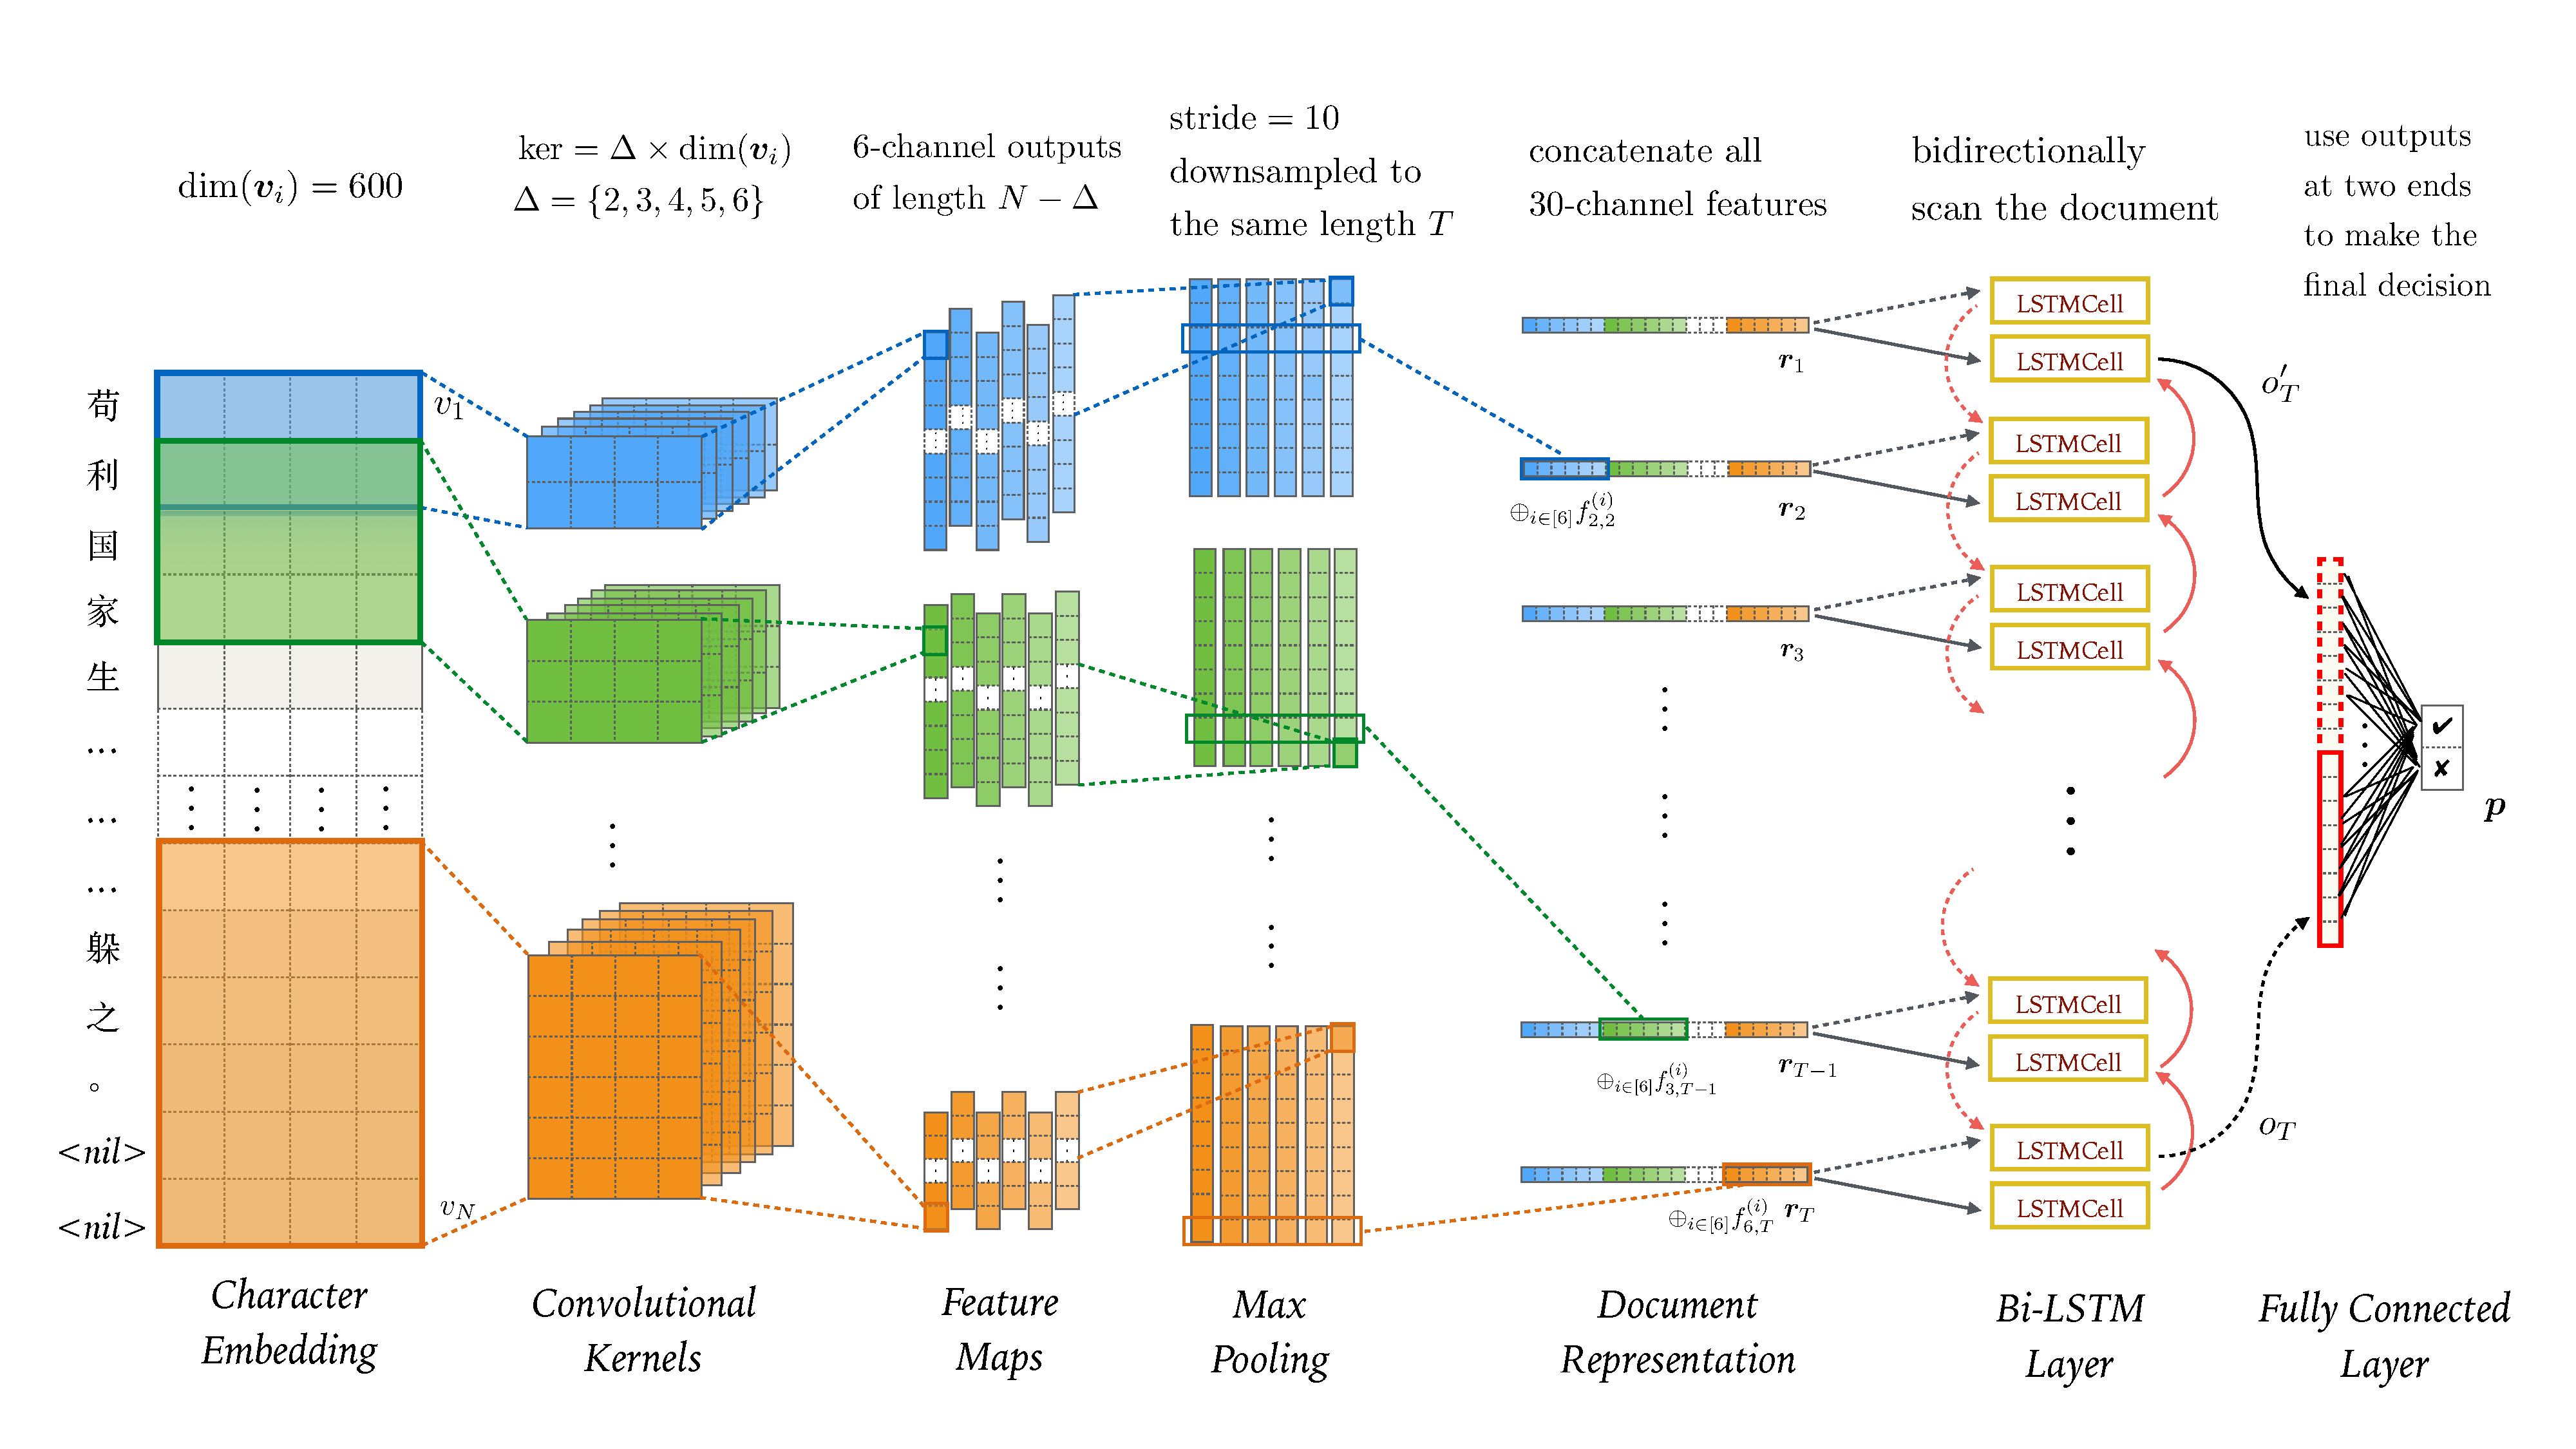
\includegraphics[width = \textwidth]{figures/model.pdf}
	\caption{Hierarchical Neural Model for Text Classification Task}
	\label{fig:model}
\end{figure}

\subsection{BiLSTM as Document Reader}
When reading, we are handling a sequential task, so it is straight forward to use recurrent neural networks. Further more, reading requires the ability to capture and memorize the context in order to understand the whole article. To incorporate memory, we use a widely used RNN variant, Bi-directional Long Short Term Memory Networks. The reason to use bi-direction here, is that human do not simply read an article from beginning to the end, but bi-directionally searching for desired information.

The BiLSTM used in our model has only one hidden layer of size 72. We concatenate the outputs $\bm o_T, \bm o'_T$ from two end to make a vector of length 144, then by a fully connected network, and then use softmax to get the final prediction.

\[\begin{cases}
	\bm o_T = \mathtt{LSTM}(\bm r_1, \bm r_2, \cdots, \bm r_T)_{T}\\
	\bm o'_T = \mathtt{LSTM}'(\bm r_1, \bm r_2, \cdots, \bm r_T)_{T}
\end{cases}, ~~\bm p = \bm W_f (\bm o_T \oplus \bm o'_T) + \bm b_f,  ~~p = \frac{exp\{\bm p_1\}}{exp\{\bm p_1\} + exp\{\bm p_2\}} \]

\section{Experiments and Results}\label{sec:exps}
\subsection{Environment}
I run the experiment on my PC. 
\begin{itemize}
	\item Operating System: CentOS Linux release 7.3.1611 (Core)
	\item CPU: Intel(R) Core(TM) i5-4460  CPU @ 3.20GHz $\times 4$
	\item No GPU
	\item Total Memory: 16142596 kB
\end{itemize}
The code is in Python 2.7 and I use PyTorch to implement neural networks.

\subsection{Training}
When training, I split the data set as training set and validation set. The validation set contains last $1000$ items and the training set contains all remaining. The minibatch is of size $64$. 

To do gradient descent, I used Adam algorithm. Although it will adapt the learning rate automatically, I manually change the learning rate from $2e-4$ to $2e-5$ after several epochs. 

The training process is extremely time-consuming. To train one epoch needs around 25 hours. Therefore my final submission is insufficiently trained.

\subsection{Results}

The AUC scores of different models I implemented evaluated on the validation are shown in Table \ref{tab:result}. I mainly compared:

\begin{itemize}
	\item FastCNN: Character vector's dimension is 400; CNN kernel size is $4\times 400$, 2 channels. Pooling stride is 20. A fully connected layer maps concatenated feature of size 148 to 2 classes (accept/reject).
	\item MultiCNN: Character vector's dimension is 200; CNN kernels are of size $2\times 200$, $3\times 200$, $4\times 200$, 2 channels each. Pooling stride is 20. A fully connected layer maps concatenated feature of size 444 to 2 classes (accept/reject).
	\item CNN+LSTM: Character vector's dimension is 120; CNN kernels are of size $2\times 120$, $3\times 120$, $4\times 120$ and $6\times 120$, 2 channels each. Pooling stride is 10. A BiLSTM with hidden size 4 to read the document representations. A fully connected layer maps concatenated feature of size 16 to 2 classes (accept/reject).
	\item Large CNN+LSTM: Change Character vector's dimension in CNN+LSTM to 400. Corresponding changes conducted to kernel size. The BiLSTM hidden layer is enlarged to the size 16.
	\item Huge CNN+LSTM: Change Character vector's dimension in CNN+LSTM to 600. Corresponding changes conducted to kernel size, add kernels of size $6 \times 600$ and add one more channel for the kernel of each size (3 channels). The BiLSTM hidden layer is enlarged to 64.
	\item Ex CNN+LSTM: Change Character vector's dimension in Huge CNN+LSTM to 128. Corresponding changes conducted to kernel size and increase the number of channel for the kernel of each size to 100 (total 500 channels). The BiLSTM hidden layer is enlarged to 72.
\end{itemize}

\begin{table}[htbp!]
\centering
\begin{tabular}{|c|c|c|c|c|c|c|c|c|c|c|c|}
\hline
	FastCNN & MultiCNN & CNN+LSTM & Large CNN+LSTM\\ 
\hline
	0.868829 & 0.869773 & 0.853858 & 0.881556\\ 
\hline\hline
	Huge CNN+LSTM & Huge CNN+LSTM 2 & Ex CNN+LSTM & Proposed HNM\\ 
\hline
	0.893592 & 0.894015 & 0.898972 & \bf 0.900659\\
\hline
\end{tabular}
\caption{Experiment results on validation set. Use a two layer neural network of hidden size 256 to stack all the 8 models in this table, we have achieved auc {\bf 0.901014} on the validation set.}\label{tab:result}
\end{table}

Our proposed Hierarchical Neural Model (HNM) outperforms all the other CNN+LSTM variants. {\bf More channels, higher embedding dimension, and larger LSTM hidden size always benefits the results} as our comparison shows. Stacking is an effective way to improve the final performance.

\section{Discussion and Future works}\label{sec:discuss}
It is a real end-to-end model, even skipping the conventional data preprocessing phase. In fact I tried the pipeline: words separation, stopping words deletion, Word2Vec pre-training, etc, to make a dataset. However, the later training process is very slow and the result is not appealing. So I abandoned this way and start to build a character level system.

The key idea of my model is to mimic the reading process of a human, which utilize the hierarchical property of documents (or language), where the CNNs act as word signal Extractors and BiLSTM acts as a high level reader. The experiment shows this structure performs much better than vanilla CNNs.

Due to the limitation of machine resource, especially the memory limit and the time restriction (I went to Spain this April. I only conducted one effective submission.), I didn't push this model to a perfect status. The final training is extremely insufficient (less than two epochs). Therefore I have to use stacked NN to integrate existing imperfect models. With enough computation resource and enough time, it is promising to use single HNM to beat the first placed integrated model in this kaggle competition.
\bibliographystyle{abbrv}
\bibliography{report}
(I think the literature review is the most arduous task of paper writing...so plz forgive such few references. On the other hand, I indeed only carefully read these three.)

\end{document}
